\chapter{Experiments and Results}

In previous chapters, we went through some basic fundamentals on how machine understands any language. From compilers that uses 0s and 1s to \acrshort{ml} models that understands the human language. In addition, we talk about few aspect about how these model became from single language models to multi-lingual models that can understand more than one language. Additionally, we talk through the multi-modality of these models that can deal with text and visual documents. Moreover, we discussed how traditional computing has changed from servers on local sites to cloud technologies. In a nutshell, we can debate about building a \acrshort{ml} models and deploying them for production use are different areas and that comes with different challenges and requirements of resources. Therefore in this chapter, we will discuss about overall performance of model and deployment separately. 

\section{Experiments and Results for Models}

As we discussed in \Cref{section_fine_tune}, when we use the \(\text{LiLT[EN-R]}_{BASE}\), which is a combination of \acrshort{lilt} with text-based model pre-trained on English language dataset, it shows higher F1 after fine-tuning for \acrfull{ser} task with compare to the model \(\text{LiLT[info-XLM]}_{BASE}\) which is a combination of \acrshort{lilt} with text-based model pre-trained on multi-lingual dataset (Please refer to \Cref{tab:compare_dataset_f1_english} and \Cref{tab:compare_datasets_f1_multilingual}). We also discussed the fine-tunning performance of both models on token classification task using English language dataset (\Cref{tab:Compare_FUNSD_token_classification}). However, all the results mentioned in \Cref{section_fine_tune} are mostly based on English language datasets, there is only one model (\(\text{LiLT[info-XLM]}_{BASE}\)) results available for \acrshort{ser} task that is fine-tuned using documents in German language (\Cref{tab:compare_datasets_f1_multilingual}). Therefore, we will combine the \acrshort{lilt} with different mono-lingual and multi-lingual text-based model to evaluate the model performance on token classification task on German language documents to find the suitable model for deployment. 

In order to find out the suitable combination for \acrshort{lilt} with different mono-lingual and multi-lingual text-based model on token classification task for German language documents, We used text-based models like RoBERTA and XLM-RoBERTA as a text-based model for text-flow. For German language documents, we used German dataset of XFUND and fine-tune all three combinations for token classification, the statistics of the dataset are described in \Cref{tab:XFUND_statistics}. In \Cref{Listing:dataset_deatures}, the dataset feature is shown, where \verb|tokens| indicates the words, \verb|bboxes| are bounding boxes, \verb|tags| are the labels associated to the word, and the image itself. The prefix of tags (\verb|'O', 'B-HEADER', 'I-HEADER'|) indicates the token position of the entity, B denotes the beginning of an entity. I indicates that token is inside the some entity. For instance if entity \verb|Empire State Building| is a \verb|B-HEADER|, entity \verb|State| will have tag \verb|I-ANSWER| which indicates that entity \verb|State| is inside the entity \verb|Empire State Building|. \verb|O| indicates that token does not correspond to any entity. 

\begin{listing}[!ht]

\begin{minted}{python}
{'id': Value(dtype='string', id=None),
'tokens': Sequence(feature=Value(dtype='string', id=None), 
          length=-1, id=None), 
'bboxes': Sequence(feature=Sequence(feature=Value(dtype='int64', id=None), 
          length=-1, id=None), length=-1, id=None),
'tags': Sequence(feature=ClassLabel(
        names=['O', 'B-HEADER', 'I-HEADER', 'B-QUESTION', 
                'I-QUESTION', 'B-ANSWER', 'I-ANSWER'], 
        id=None
        ), 
        length=-1, 
        id=None),
'image': Image(decode=True, id=None)}    
    
\end{minted}

\caption{Dataset features}
\label{Listing:dataset_deatures}   
\end{listing}

In order to find out the model performance we have used seqeval\footnote{\url{https://huggingface.co/spaces/evaluate-metric/seqeval}, Accessed: 28.04.2024}. seqeval is a Python framework for evaluation of labeling task. The fundamental of seqeval is similar to confusion matrix (\Cref{tab:Confusion Matrix}). It takes two mandatory arguments like prediction and references. The output of this matrix is the scores like accuracy, precision, recall and F1. An example of the functionality of the metric seqeval is shown in \Cref{Listing:seqeval_example}, in this example the predictions and references are same hence it is in "full match" case, therefore the average precision, recall, accuracy and f1 will be 1. If the predictions and references are not same, then the case will be "no match" and the average output results will be 0. 

\begin{listing}[!ht]

\begin{minted}{python}
>>> seqeval = evaluate.load('seqeval')
>>> predictions = [['O', 'O', 'B-HEADER', 'I-HEADER', 'I-HEADER', 'I-HEADER', 'O']]
>>> references = [['O', 'O', 'B-HEADER', 'I-HEADER', 'I-HEADER', 'I-HEADER', 'O']]
>>> results = seqeval.compute(predictions=predictions, references=references)
>>> print(results)
{
    'overall_precision': 1.0, 
    'overall_recall': 1.0, 
    'overall_f1': 1.0, 
    'overall_accuracy': 1.0
} 
    
\end{minted}

\caption{An Example of Seqeval}
\label{Listing:seqeval_example}   
\end{listing}

\subsection{Fine-tuning results for 30 epoch}
We have used text-besed models like RoBERTa and XLM-RoBERTa in order to combine it with \acrshort{lilt}. RoBERTa is a text-based model that has been pre-trained on English language dataset and XLM-RoBERTa is pre-trained on multi-lingual dataset. We started with 30 epoch to see the results of these models in combination with \acrshort{lilt} on German language dataset for token classification task since the fine-tuning of these model takes large amount of computing resources. The fine-tuning results of \acrshort{lilt} for 30 epoch with different combination of text-based model over German language dataset for token classification task is shown in \Cref{tab:30_epoch_results}. In this setting, the mono-lingual text-based models in combination with \acrshort{lilt} shows higher overall scores with compare to multi-lingual text-based model. The classification results of \(\text{LiLT[En-R]}_{BASE}\) on all classes(\ref{multi_class}) is described in \Cref{fig:multi_calss_en_lilt}, The model performance on classes \verb|HEADER, QUESTION, ANSWER|  are described in \Cref{Listing:main_Classes_res_30_epoch}. However, in table, we saw \(\text{LiLT[InfoXLM]}_{BASE}\) shows overall f1 of 0.823 for \acrshort{ser} task on German language dataset. Therefore, we also include  \(\text{LiLT[InfoXLM]}_{BASE}\) for token classification task on German language dataset to compare the fine-tune results between two multi-lingual text-based models. We can see that the model pre-trained on multi-lingual dataset (XLM-RoBERTa and InfoXLM) shows nearly identical results. 

\begin{table}[!ht]
    \centering
    \captionsetup{justification=centering}
    \begin{tabular}{lcccl}
        \toprule
        \textbf{Model}& \textbf{Precision}& \textbf{Recall}& \textbf{F1} & \textbf{Accuracy}\\ \midrule
        \(\text{LiLT[InfoXLM]}_{BASE}\)& 0.378& 0.537& 0.444& 0.636 \\ \midrule
         \(\text{LiLT[En-R]}_{BASE}\) &  0.744& 0.795& 0.768& 0.756 \\
         \(\text{LiLT[XLM-RoBERTa]}_{BASE}\)& 0.359& 0.535& 0.430& 0.627 \\ \bottomrule
    \end{tabular}
    \caption{Fine-tuning results of \acrshort{lilt} in combination with different text-based models on German language dataset for token classification task over 30 epoch}
    \label{tab:30_epoch_results}
\end{table}

\begin{listing}[!ht]

\begin{minted}{python}
{
0: 'O', 
1: 'B-HEADER', 
2: 'I-HEADER', 
3: 'B-QUESTION', 
4: 'I-QUESTION', 
5: 'B-ANSWER', 
6: 'I-ANSWER'
}
\end{minted}
\caption{Labels Assigned to number}
\label{multi_class}
\end{listing}


\begin{listing}[!ht]
\captionsetup{justification=centering}
\begin{minted}{python}
    'ANSWER':  {'precision': 0.78515625, 'recall': 0.7905604719764012,
                'f1': 0.7878490935815776, 'number': 1017},
    'HEADER':  {'precision': 0.6, 'recall': 0.46551724137931033,
                'f1': 0.5242718446601942, 'number': 58},
    'QUESTION':{'precision': 0.7019464720194647, 'recall': 0.8290229885057471,
                'f1': 0.7602108036890646, 'number': 696}
\end{minted}
\caption{Results on Classes \(\text{LiLT[En-R]}_{BASE}\)(\Cref{tab:30_epoch_results}), \\ fine-tuned-language: German, Evaluation-dataset-language:German }
\label{Listing:main_Classes_res_30_epoch}
\end{listing}

\begin{figure}[!ht]
    \centering
    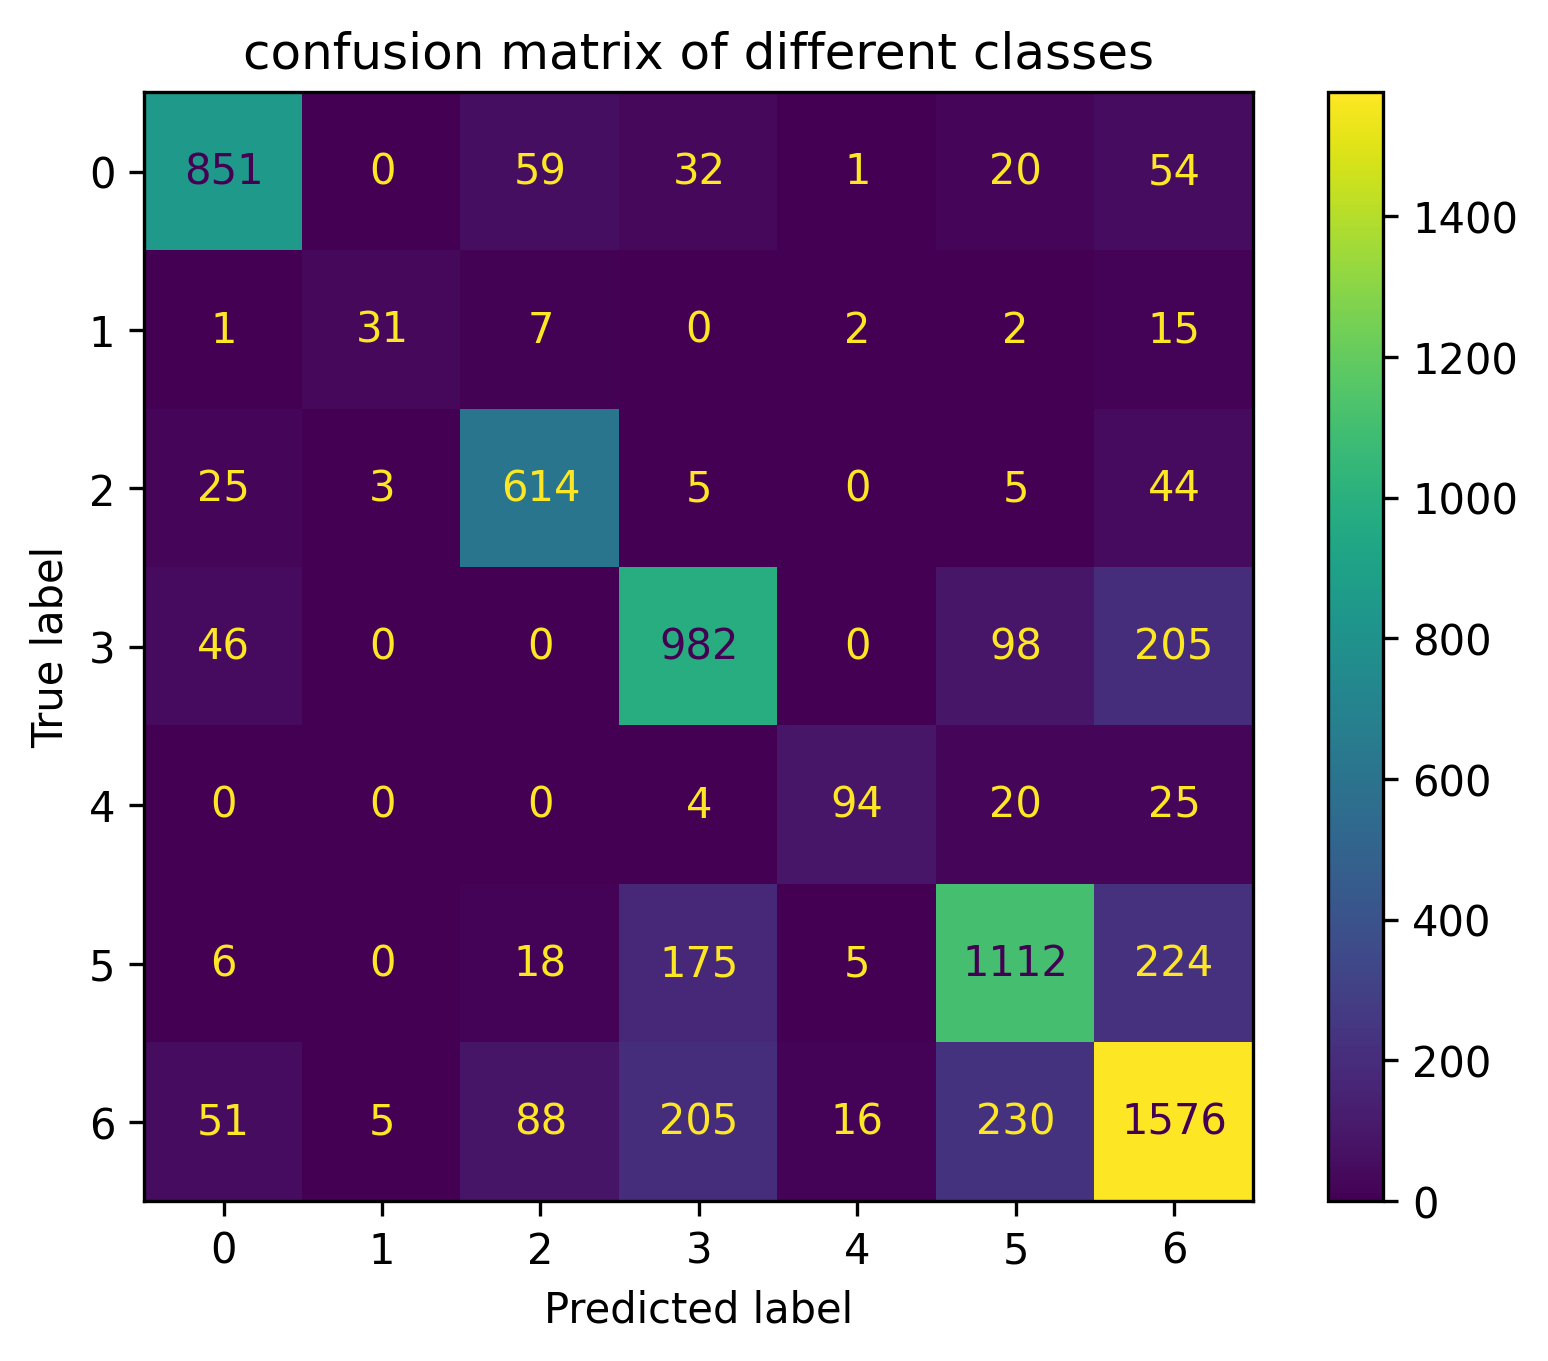
\includegraphics[width=0.6 \textwidth]{chapters/images/experiments_and_results/En_LiLT_30_output.png}
    \caption{Confusion matrix of all classes using \(\text{LiLT[En-R]}_{BASE}\) from \Cref{tab:30_epoch_results} }
    \label{fig:multi_calss_en_lilt}
\end{figure}
    
% \begin{figure}[H]
%     \centering
%     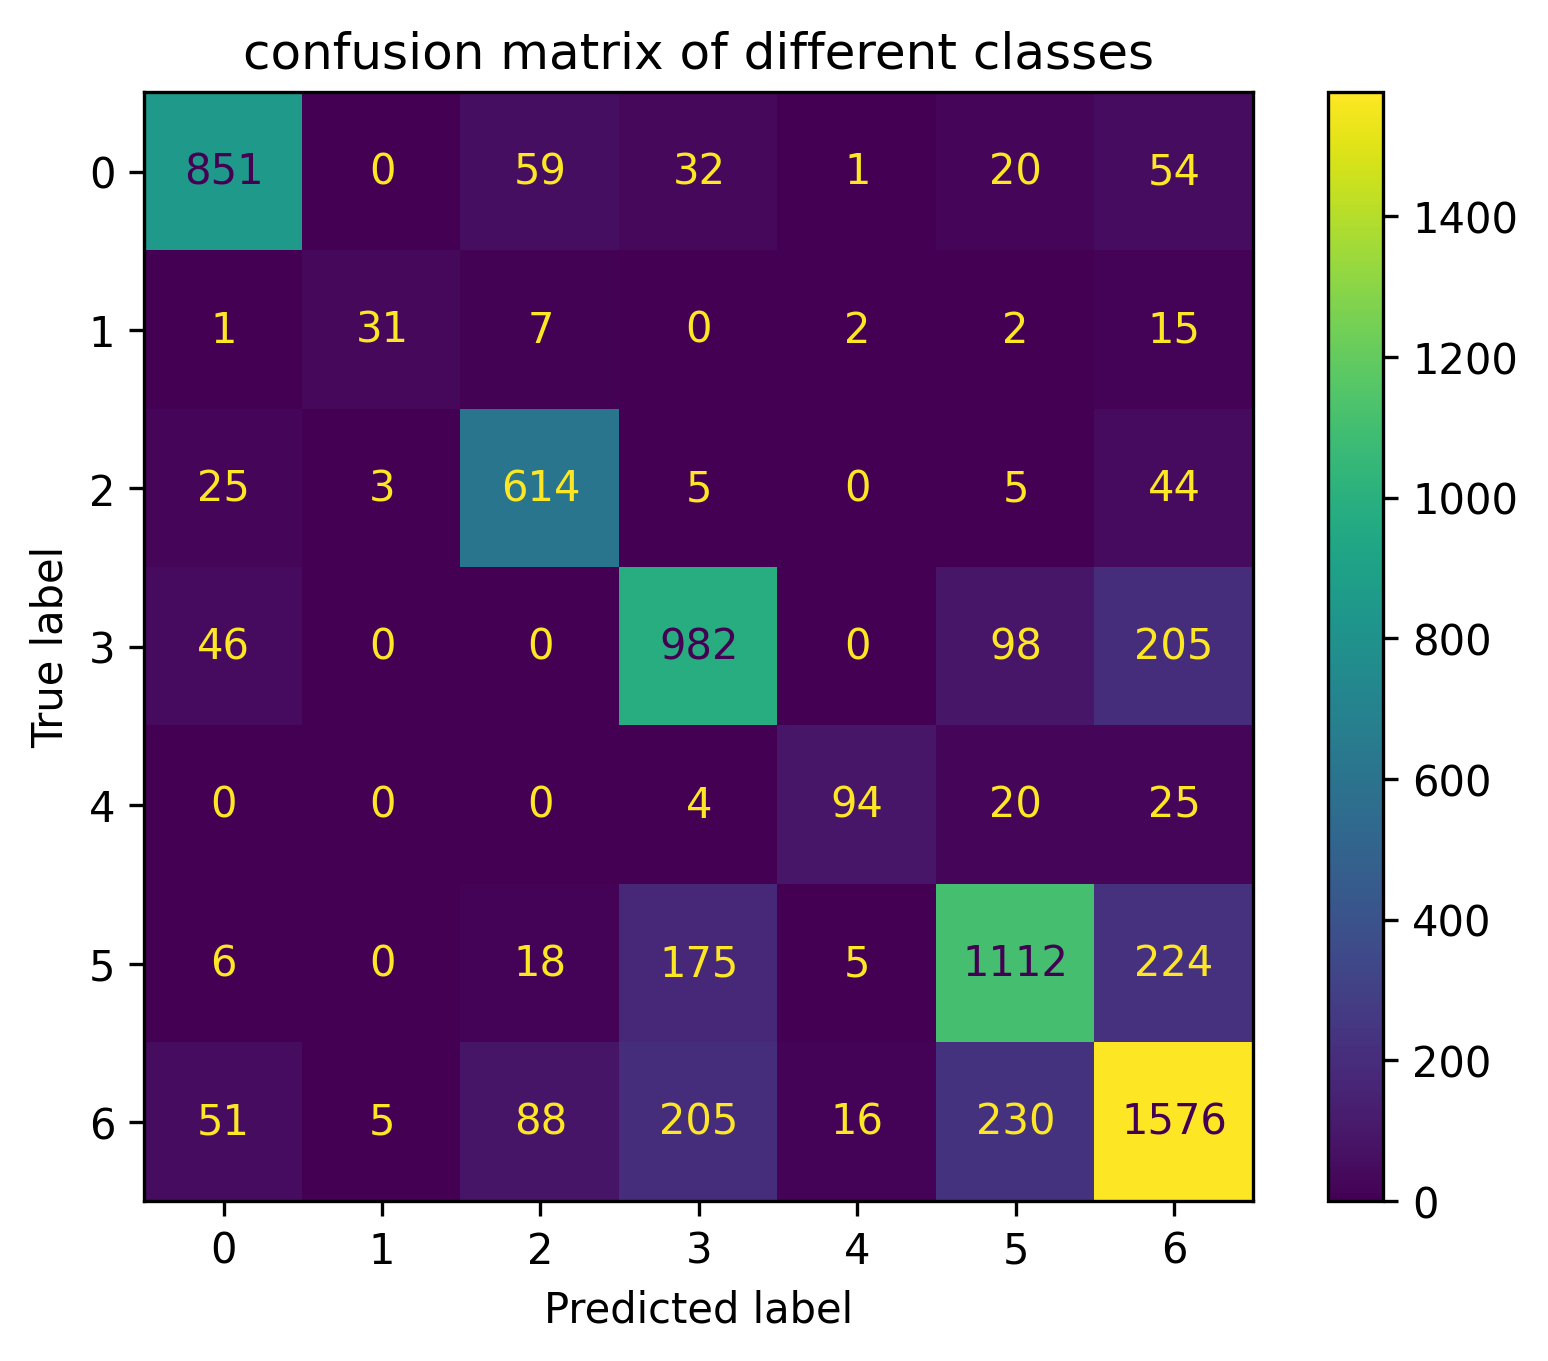
\includegraphics[width=0.6 \textwidth]{chapters/images/experiments_and_results/En_LiLT_30_output.png}
%     \caption{Confusion matrix of all classes using \(\text{LiLT[En-R]}_{BASE}\) from \Cref{tab:30_epoch_results} }
%     \label{fig:multi_calss_en_lilt}
% \end{figure}





\subsection{Fine-tuning result of LiLT for 100 epoch}
Due to the high demand of resource and computing power needed to fine-tune these models for 100 epoch, it is time consuming and costly to fine-tune all the models over large number of training cycles. For instance, it took almost 2 and a half day to fine-tune \(\text{LiLT[XLM-RoBERTa]}_{BASE}\) using Intel Core i7-1185G7 Processor\footnote{\url{https://www.intel.com/content/www/us/en/products/details/processors/core.html}, Accessed: 3.5.2024}. If we want to use the same settings and fine-tune the model using AWS EC2, It would cost around \$ 30 for each training using models in the BASE settings. However, as the size of the model rises, the cost rises dramatically making it a key concern to choose right resources and methods to choose to cut down the cost before the training. According to the \Cref{tab:Compare_FUNSD_token_classification}, for English language dataset, LiLT[XLM-RoBERTa] achieves F1 score of 0.735 within 20 epoch, where the same model shows 0.430 F1 for German language dataset on token classification within 30 epoch(\Cref{tab:30_epoch_results}). Moreover, LiLT[EN-R] reaches 0.771 F1 for 50 epoch and the highest 0.806 over 106 epoch, on other hand the same model for German language dataset reached 0.76 F1 within 30 epoch(\Cref{tab:30_epoch_results}). The combination of English-RoBERTa shows good performance in both the dataset (English and German) within less number of epochs. Since InfoXLM and XLM-RoBERTa are pre-trained on multi-lingual dataset and both shows almost similar performance for 30 epoch, therefore we kept one type of model (RoBERTa) for large amount of training to save time and cost over computing resources. We fine-tuned LiLT[XLM-RoBERTa] and LiLT[EN-R] for 100 epoch on German language dataset for token classification task and achieved 0.707 F1 for LiLT[XLM-RoBERTa] and LiLT[EN-R] overall F1 was 0.763, The results of the metric are shown in \Cref{tab:100_epoch_results}. In \Cref{fig:Multi-class_XLM}, the confusion matrix for all classes is described for LiLT[XLM-RoBERTa],  LiLT[EN-R] fine-tuned with 30 epochs shows better results than with 100 epochs, the confusion matrix for different classes and overall results for LiLT[EN-R] is described in \Cref{fig:multi_calss_en_lilt} and \Cref{tab:30_epoch_results}. In \Cref{fig:Multi-class_XLM}, the numbers in axis represents the labels as shown in \Cref{multi_class}.


\begin{table}[!ht]
    \centering
    \captionsetup{justification=centering}
    \begin{tabular}{lcccl}
        \toprule
        \textbf{Model}& \textbf{Precision}& \textbf{Recall}& \textbf{F1} & \textbf{Accuracy}\\ \midrule
         \(\text{LiLT[En-R]}_{BASE}\) &  0.743& 0.783& 0.763& 0.752 \\
         \(\text{LiLT[XLM-RoBERTa]}_{BASE}\)& 0.686& 0.728& 0.707& 0.757 \\ \midrule
    \end{tabular}
    \caption{Fine-tuning results of \acrshort{lilt} in combination with different text-based models on German language dataset for token classification task over 100 epoch}
    \label{tab:100_epoch_results}
\end{table}



\begin{figure}[!ht]
    \centering
    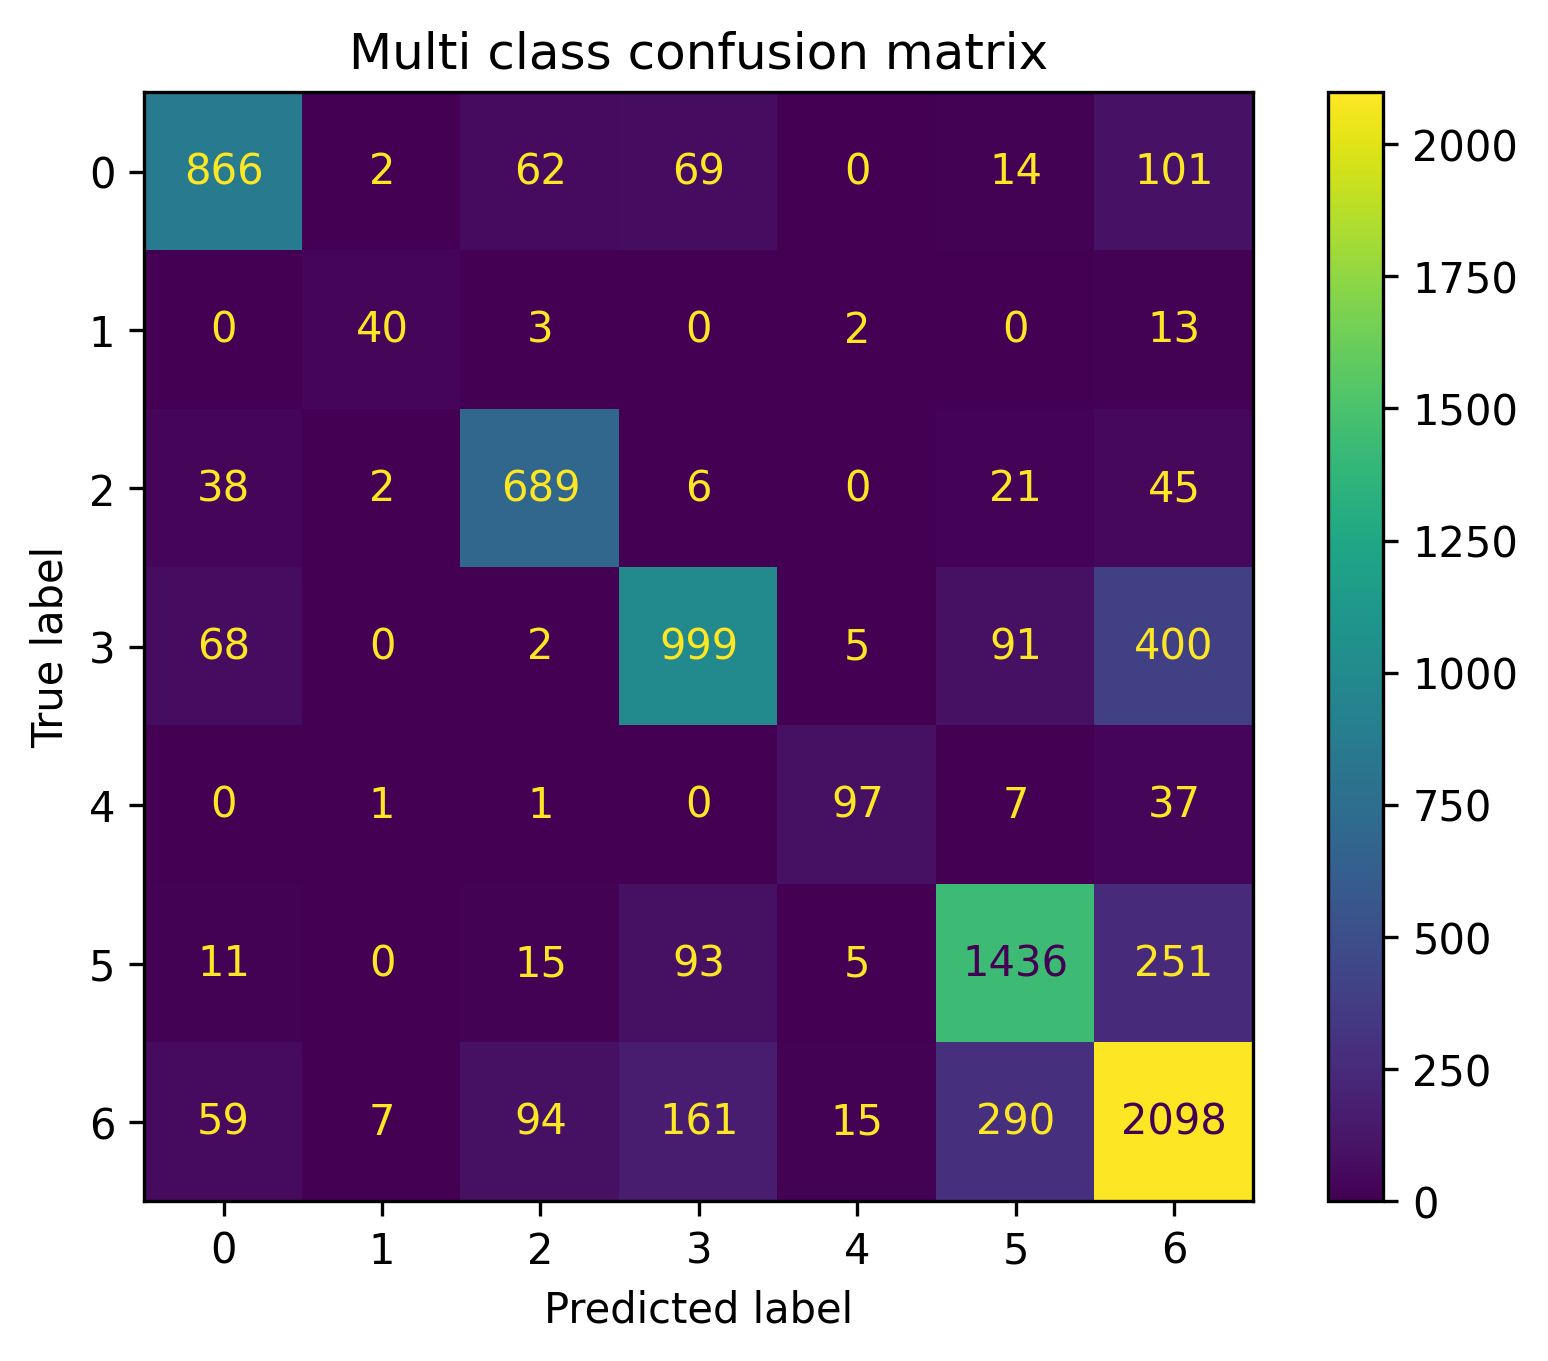
\includegraphics[width=0.6 \textwidth]{chapters/images/experiments_and_results/XLM_100_output.png}
    \caption{Confusion matrix of all classes(\ref{multi_class}) using \(\text{LiLT[XLM-RoBEERTa]}_{BASE}\) from \Cref{tab:100_epoch_results}}
    \label{fig:Multi-class_XLM}
\end{figure} 

\subsection{Results of Fine-tuned LiLT in German language with other Languages}
Pre-training and Fine-tunning are crucial steps in \acrshort{nlp}, during the pre-training, the model learns about linguistic structures, grammar and semantic understanding at some level. As we discussed \acrshort{lilt} can be used in combination with text-based models like RoBERTa and XLM-RoBERTa, where RoBERTa is pre-trained using English language and XLM-RoBERTa is pre-trained using around 100 languages. While in fine-tuning on specific task such as token classification, model adapt its general knowledge from pre-traing to the spcific tasks. The combinations of pre-trained \acrshort{lilt} with EN-RoBERTa and XLM-RoBERTa are available at GitHub\footnote{\url{https://huggingface.co/nielsr}, Accessed: 03.05.2024 \label{base_models}} that are pre-trained using FUNSD dataset which is an English language dataset. As we discussed above, We used LiLT[EN-R] and LiLT[XLM-RoBERTa] and fine-tuned for token classification task using German language dataset, the model shows good results on German language datasets since its been fine-tuned on German language and weights are adapted to that language. At this point, both model's weights are first changed while pre-training using FUNSD and fine-tuning using German language dataset. In addition, during fine-tuning the layout information is also being added to the model's knowledge. We have used XFUND dataset that is having 7 languages to compare the results of LiLT[XLM-RoBERTa] pre-trained on FUNSD and LiLT[XLM-RoBERTa] fine-tuned on token classification task using German language dataset. Since, the XFUND dataset was missing features like "\verb|words|" of the documents, instead XFUND comes with "\verb|input_ids|" feature and using multi-lingual tokenizer for LiLT[EN-R] was not possible. Therefore, LiLT[EN-R] was excluded from the evaluation for XFUND dataset except German since there is a German language subset of XFUND avaialable at Hugging face hub\footnote{\url{https://huggingface.co/datasets/cooleel/xfund_de}, Accessed: 05.05.2024} that have features like \verb|words| of each documents and therfore there was a possibility to include LiLT[EN-R] for German and English language. In table, the evaluation results of fine-tuned LiLT[EN-R] in German language for token classification task is shown in \Cref{tab:EN_R_on_different_languages} and the evaluation results of LiLT[XLM-RoBERTa] on different languages are described in \Cref{tab:Eval_on_different_language}. 


\begin{table}[!ht]
    \centering
    \begin{tabular}{lccccl}
        \toprule
         \textbf{Dataset}& \textbf{Language}& \textbf{Precision}& \textbf{Recall}& \textbf{F1} & \textbf{Accuracy}  \\ \midrule
         FUNSD & EN & 0.52641 & 0.41082 & 0.46149 & 0.54629\\
         XFUND & DE &  0.74457 & 0.79503 & 0.76897 & 0.75618 \\ \bottomrule
    \end{tabular}
    \caption{Comparison of fine-tuned LiLT[EN-R] in German language documents with different languages}
    \label{tab:EN_R_on_different_languages}
\end{table}


\begin{table}[!ht]
    \centering
    \begin{tabular}{lccccl}
    \toprule
    \textbf{Dataset}& \textbf{Language} & \textbf{Precision} &\textbf{Recall} & \textbf{F1} & \textbf{Accuracy}\\ \midrule
    \multirow{7}{*}{XFUND} &FR  &0.00392  & 0.00952 &0.00555  &0.247  \\
                  &  ES&0.00279  &0.00724  &0.00403  &0.21296  \\
                  & IT& 0.00478 & 0.01193 & 0.00683 & 0.19410\\
                  & PT & 0.00429 & 0.00885 & 0.00578 & 0.20010\\
                  & JA & 0.00324 & 0.00766 & 0.00455 & 0.29468 \\
                  & ZH & 0.00456 & 0.00821 & 0.00586 & 0.18616\\
                  &DE & 0.68672& 0.72715&  0.70715& 0.75766 \\  \midrule
                FUNSD  & EN& 0.37032 & 0.32297 & 0.34503 & 0.49394\\ \bottomrule
                  
    % \multirow{2}{*}{FUNSD} & \(\text{EN}_{\text{LiLT[EN-R]}}\) & 0.52641 & 0.41082 & 0.46149 & 0.54629\\
    %                         & EN& 0.37032 & 0.32297 & 0.34503 & 0.49394\\ \midrule
    % \multirow{2}{*}{XFUND} & \(\text{DE}_{\text{LiLT[EN-R]}}\) & 0.74457 & 0.79503 & 0.76897 & 0.75618 \\
                                
    \end{tabular}
    \caption{Comparison of fine-tuned LiLT[XLM-RoBERTa] in German language documents with different languages}
    \label{tab:Eval_on_different_language}
\end{table}



% \subsection{Results of Fine-tuned LiLT in German language with English Language}
% \acrshort{lilt} is pre-trained over English language dataset FUNSD, the pre-trained model have the knowledge about linguistic structures, grammer, layouts in documents and some level of semantic understanding. When its been fine-tuned in German language documents using German language subset from XFUND, the weights of the models adjusted to specific task for instance token classification in German language documents in our case. This will allow the model to apply the knowledge it learned during the pre-training to the new context. To evaluate the performance of \acrshort{lilt} that is pre-trained in English and fine-tuned in German on English language dataset, we used FUNSD. The evaluation results over an English language dataset is described in table. 

 % In order to form a hypothesis to evaluate fine-tuned model, there are things like language and layout should be included. However, fine-tuning the model over 7 languages needs more time and resources. Therfore, we decided to first evaluate the pre-trained models over XFUND dataset on 7 different languages. Second, evaluate our model on XFUND dataset on 7 different languages. Note that in both the approach models are pre-trained on one language only. So it is not surprising that the model that is not fine-tune for specific task will perform worst in that tasks. On other hand the model is fine-tune for that specific task will perform good in that specif task but it will show worst performance in the languages that the model has never seen. Therfore, our goal for this experiment is to find out how layout information can help model to be independent from the language.